\chapter[\small LA RECONNAISSANCE FACIALE PAR LES M\'{E}THODES EIGENFACE ET LBP]{LA RECONNAISSANCE FACIALE PAR LES MÉTHODES EIGENFACE ET LBP}
\section{Introduction}
La reconnaissance de visage est sans doute le moyen le plus utilisé au quotidien pour identifier un  membre de son entourage. La reconnaissance automatique de visage s'inscrit dans le domaine vaste la de vision par ordinateur qui part du constat selon lequel le sens le plus utilisé chez l'homme est la vue. Dès lors, il peut s'avérer important de \og donner les yeux à son ordinateur\fg{} : ainsi il pourra remplacer l'homme dans les tâches répétitives de reconnaissance faciale. Parmi les différentes méthodes présentées au chapitre précédent, certaines ont l'avantage d'être rapide, facile à mettre en œuvre ou ont un taux élevé de reconnaissance. Dans ce chapitre, nous présentons dans un premier temps la méthode de reconnaissance eigenface, puis dans un second temps l'approche LBP(Local Binary Patterns). 
\section{Reconnaissance par eigenface}

\subsection{présentation de la méthode eigenface}
L'algorithme PCA ou eigenface s'appuie sur des propriétés statistiques et utilise l'algèbre linéaire pour classifier les visages. C'est l'un des algorithmes les plus utilisés car il est relativement facile à mettre en œuvre et est à la base de nombreux autres algorithmes. Ses principaux inconvénients c'est sa sensibilité aux problèmes d'éclairage, de pose et d'expressions faciales.

L'approche eigenface consiste à représenter un visage $\Phi_{i}$ comme une combinaison linéaire d'un ensemble d'images 
M, ces dernières formant ainsi une base de référence. Mathématiquement, cela revient à établir l'équation \ref{eq5} : 
\begin{eqnarray}
\Phi_{i}=\sum_{i=1}^{n}{p_id_i}
\label{eq5}
\end{eqnarray}
où $d_i$ représente le visage propre, et $p_i$ le coefficient associé.

Pour calculer les $p_i$ représentant les poids, on traite une image $I_i(m,n)$ comme un vecteur $\Gamma_(m\times n,1)$ dans un espace vectoriel de plus grande dimension $N=m \times n$, par concaténation de colonnes.

\[
   I_i(m,n)=\begin{pmatrix}
\alpha_{11} & \alpha_{12}& \ldots & \alpha_{1n}\\
\alpha_{21} & \alpha_{22}& \ldots & \alpha_{2n}\\
\ldots& \vdots& \vdots & \vdots        \\
\alpha_{m1} & \alpha_{m2}& \ldots & \alpha_{mn}
\end{pmatrix}\]

est transformée en

\[\Gamma_i(m\times n,1)= \begin{pmatrix}
\alpha_{11} \\
\alpha_{12} \\
\vdots     \\
\alpha_{1n}   \\
\alpha_{21}   \\
\alpha_{22}  \\
\vdots   \\
\alpha_{2n}  \\
\vdots        \\
\alpha_{m1} \\
\alpha_{m2}\\
\vdots \\
\alpha_{mn}
\end{pmatrix} 
\]
Les coefficients $\alpha_{i,j}$ représentent les valeurs des pixels en niveau de gris, codés de 0 à 255.
On peut alors rassembler les M images d'apprentissage dans une unique matrice, nous obtenons une matrice d'images $\Gamma$, où chaque colonne représente une image $\Gamma_i$.
\[\Gamma= \begin{pmatrix}
\alpha_{11} &\beta_{11} &\ldots&\zeta_{11}\\
\vdots      &\vdots     &\ldots&\vdots\\
\alpha_{1n} &\beta_{1n}&\ldots&\zeta_{1n} \\
\alpha_{21} &\beta_{21} &\ldots&\zeta_{21} \\
\vdots      &\vdots     &\ldots& \vdots  \\
\alpha_{2n} &\beta_{2n} &\ldots&\zeta_{2n} \\
\vdots      & \vdots    &\ldots&\vdots    \\
\alpha_{m1} &\beta_{m1} &\ldots&\zeta_{m1} \\
\vdots      &\vdots     &\ldots&\vdots \\
\alpha_{mn} &\beta_{mn} &\ldots&\alpha_{mn}
\end{pmatrix} 
\]

On peut alors déduire le visage moyen par la formule 
\begin{eqnarray}
\Psi=\frac{1}{M}\sum_{i=1}^{M}{\Gamma_i}
\label{eq6}
\end{eqnarray}
A chaque visage d'apprentissage, on soustrait le visage moyen de la manière suivante.
\begin{eqnarray}
\phi_i=\Gamma_i -\Psi
\label{eq7}
\end{eqnarray}
$i=1, 2,\ldots, M$ où $\phi_i$ représente le $i^{ème}$ visage auquel on a soustrait le visage moyen.

 On obtient alors les informations propres à ce visage. Dès lors on peut calculer la matrice de covariance D. Elle correspond à
\begin{eqnarray}
D=QQ^{t}
\label{eq8}
\end{eqnarray}
où $Q=\begin{pmatrix} \phi_1&\phi_2 &\ldots&\phi_M\end{pmatrix}$.

L'étape suivante est le calcul des valeurs propres $d_i$ de la matrice $D$. Comme la matrice $D$ est carrée d'ordre $n\times m$, on aura également $n\times m$ vecteurs propres de dimension $n\times m$ chacun. Il peut s'avérer difficile et très long de les calculer. La solution consiste à réduire la dimension de l'espace de travail. Nous allons donc considérer la matrice $E=Q^tQ$ et trouver ses valeurs propres. Par  exemple \citep{SAB}, pour 50 images de résolution $180\times200$, nous pourrions résoudre une  matrice L de $50\times50$ au lieu d'une matrice de $36000\times 36000 $ pour ensuite prendre les  combinaisons  linéaires  appropriées  des  images $\phi_i$. Cette opération permet de passer d'une complexité de l'ordre du nombre de pixel de l'image à une complexité de l'ordre du nombre d'image. Le passage de la matrice D à la matrice E est justifié par le fait que les vecteurs propres de ces deux matrices sont liés de manière assez proche.

En effet 
\begin{eqnarray}
Ee_i=Q^tQe_i=\lambda_ie_i
\label{eq9}
\end{eqnarray}
avec $\lambda_i$ la valeur propre associé au vecteur propre $e_i$.\\
En multipliant l'équation \ref{eq9} par la matrice Q, il ressort :
\begin{eqnarray}
QEe_i=QQ^tQe_i
\label{eq10}
\end{eqnarray}
soit \begin{eqnarray*}
QEe_i=DQe_i=Q\lambda_ie_i
\label{eq11}
\end{eqnarray*}
Donc si $e_i$ est un vecteur propre de la matrice E associé à une valeur propre $\lambda_i$, alors $Qe_i$ est un vecteur propre de la matrice D associé à la même valeur propre $\lambda_i$. Ainsi, nous avons $d_i$ vecteur propre de D, avec \begin{eqnarray}
d_i = Qe_i
\label{eq12}
\end{eqnarray}
Nous pouvons donc trouver les valeurs propres de l'énorme matrice D en trouvant 
d'abord les valeurs propres de la matrice E beaucoup plus petite, puis pour trouver les vecteurs propres de D, il suffit juste de multiplier les vecteurs propres de E par la matrice Q. Une fois les vecteurs propres trouvés, on les classe selon leurs valeurs propres associées et de manière décroissante. Puisque les valeurs propres les plus grandes renferment le plus d'informations, on va sélectionner les k meilleures valeurs propres (les plus significatifs). On définit alors un espace vectoriel engendré par ces $k$ vecteurs propres, que 
l'on appelle l'espace des visages $E_v$ ou \og Face Space\fg{}. Une image originale est alors un vecteur de cette espace vectoriel(c'est-à-dire s'écrit comme combinaison linéaire des vecteurs propres). La figure \ref{fig:eigenface} montre un exemple de faces propres.

Dans la pratique, on choisit k selon un pourcentage $\gamma$ tel que
\begin{eqnarray}
\frac{\sum_{i=k+1}^{n}\lambda_i}{\sum_{i=1}^{n}\lambda_i} < \gamma
\label{eq13}
\end{eqnarray}
où $n$ représente le nombre total de valeurs propres.
Les \og k \fg{} premiers vecteurs propres correspondant aux \og k \fg{} plus grandes valeurs doivent être convenablement choisies car constituent un paramètre  critique  sur  lequel  dépend  la  performance  du  système  de reconnaissance. 
\subsection{Processus de reconnaissance par eigenface}
Pour classifier un visage par eigenface, on projecte d'abord les images d'apprentissage sur l'espace des visages $E_v$. Une image $\Gamma_i$ est alors transformée en ses \og composantes Eigenfaces\fg{} par une simple opération de projection vectorielle.
 \begin{eqnarray}
p_i&=&d_i^t\phi_i\\
   &=&d_i^t(\Gamma_i -\Psi)
\label{eq14}
\end{eqnarray}pour $i=1,2, \ldots, k$.

Les  vecteurs $p_i$ sont  appelés  vecteurs  de  poids  et  forment  une  matrice 
$\Pi=\begin{pmatrix} p_1&p_2 &\ldots& p_k\end{pmatrix}$  qui  décrit  la  contribution  de  chaque  eigenface  dans  la  représentation  de l'image  d'entrée. La  matrice $\Pi$ est  alors  utilisée  pour  trouver  quelle  est,  parmi  un  nombre 
prédéfini de classes, celle qui décrit le mieux une image d'entrée.

La méthode la plus simple pour déterminer quelle classe de  visage fournit la meilleure
description d'une image d'entrée est de trouver la classe de visage $k$ qui minimise la distance euclidienne.
\begin{eqnarray}
\epsilon_k^2=\left\|\Pi-\Pi_k\right\|
\label{eq15}
\end{eqnarray}
Les étapes suivantes résume la techniques d'eigenfaces.

La phase d'apprentissage comprends :


\begin{itemize}
	\item [\textbullet] la collecte  des  M  images  faciales  et  construction  de  la  matrice  $\Gamma$, par concaténation des colonnes des images faciales. 
		\item [\textbullet]  le calcul du visage moyen en sommant les colonnes de la matrice $\Gamma$ et en divisant le vecteur résultant par le nombre d'image d'entrée M ( voir \ref{eq6}).
     \item [\textbullet] la soustraction du visage moyen de la matrice $\Gamma$ pour obtenir la matrice $Q$ ; où chaque élément représente la variance des valeurs d'intensité de chaque pixel.
		\item [\textbullet] le calcul de la matrice $E=Q^tQ$,
		\item [\textbullet] le calcul des vecteurs propres de $E$ puis leur tri dans un ordre descendant selon les valeurs propres associées.
		\item [\textbullet] le calcul  des  vecteurs  propres  de  la  matrice  de  covariance $C^t$  et  obtention  des  visages propres en multipliant les vecteurs propres de $E$ par la matrice $Q$.
		\item [\textbullet] le choix des $k$ meilleurs valeurs propres et les vecteurs propres associés.
		\item [\textbullet] la détermination du poids des images d'entrée en projetant chaque image dans l'espace
visage.
\item [\textbullet] la sauvegarde du visage moyen, les eigenfaces et la matrice de projection (de poids) des images.
\end{itemize}

Les 9 étapes ci-dessus transforment une base de données images en un ensemble de projection dans l'espace visage.

L'étape de reconnaissance comprends : 
\begin{itemize}
	\item [\textbullet] le prétraitement de l'image d'entrée et soustraction du visage moyen,
	\item [\textbullet] la détermination du poids de l'image d'entrée par la projection de celle–ci dans l'espace 
visage en multipliant le vecteur résultant de la première étape d'apprentissage par les eigenfaces de la base de données.
  \item [\textbullet]la mesure de la similarité  en  utilisant  des  métriques  telles  que  la  distance euclidienne.
	\end{itemize}
	
	NB. Plusieurs métriques peuvent être utilisés pour mesurer la similarité de deux vecteurs $X=(x_1,x_2,\ldots,x_n)$ et $Y=(y_1,y_2,\ldots,y_n)$ à l'instar de la distance euclidienne $$d(X,Y)=\sqrt{\sum_{i=1}^{n}{\left|x_i-y_i\right|^2}}$$ la distance de City-Block (ou de Manathan) $$d(X,Y)=\sum_{i=1}^{n}{\left|x_i-y_i\right|}$$ la distance de Mahalanobis (cf. \cite{KATO}).
	
	Toutefois, le choix de la mesure est parfois difficile et est souvent argumenté par rapport à l'espace d'attributs.
	
\section{Reconnaissance par la méthode des Local Binary Patterns} 
\subsection{Présentation de la méthode LBP}
La méthode LBP telle que décrite par Ahonen et al. dans \cite{TIM} prend en entrée un carré de  9 pixels et a pour sortie un nombre binaire 8 bits. Les auteurs ont été motivés par le fait qu'un visage peut être vu comme un assemblage de micro-patterns dont la description par LBP est à la fois bonne, robuste face aux variations de gris et rapide à générer. 

\begin{figure}[htbp]
	\centering
		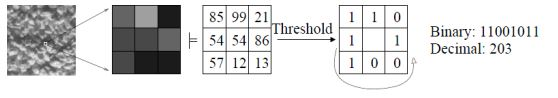
\includegraphics{BLP.JPG}
	\caption[opérateur LBP ]{opérateur LBP \textit{(source :\cite{TIM})}}
	\label{fig:LBP}
\end{figure}

Un seuil est appliqué tel que tous les pixels périphériques dont la valeur est supérieure à la valeur du pixel central se voient attribuer la valeur 1 tandis que les autres reçoivent la valeur 0. La valeur LBP est obtenue en lisant autour du pixel central dans le sens trigonométrique (comme indiqué dans la figure \ref{fig:LBP}. Pour convertir toute l'image, on déplace le carré de conversion $3\times 3$ sur l'ensemble de l'image.

Pour rester fiable, l'opérateur LBP a été étendue.  Dans ce cas, un cercle de rayon R autour du pixel central et les valeurs des P points échantillonnés sur le bord de ce cercle sont prises et comparées avec la valeur du pixel central (voir figure \ref{fig:lbpam} tirée de \cite{TIM} ). Cet entourage sera notée $(P,R)$. Comme ces P points ne tombent pas nécessairement
au centre d'un pixel de l'image, leurs valeurs sont obtenues par interpolation bilinéaire \cite{TIM}.
\begin{figure}[htbp]
	\centering
		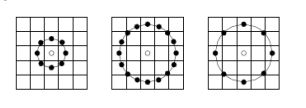
\includegraphics{lbpam.JPG}
	\caption[LBP étendue]{LBP étendue \textit{(source :\cite{TIM})}}
	\label{fig:lbpam}
\end{figure}

Dans la figure \ref{fig:lbpam} sont représentés les entourages $(8,1)$, $(16,2) $et $(8,2)$. Dans cette nouvelle représentation ne sont gardés que les patterns uniformes. Un pattern est dit uniforme s'il ne présentent pas plus de deux transitions '0-1' ou '1-0' et de manière circulaire. Ainsi 00110000 et
10000001 sont uniformes tandis que 10010001 et 10011101 ne le sont pas. Ojala et al. \cite{OJA} ont montré que les  LBPs  uniformes contiennent plus de 90\% de l'information d'une image. L'utilisation d'un code LBP uniforme, noté LBPu2 à deux avantages. Le premier est le  gain  en  mémoire  et  en  temps  calcul.  Le  deuxième  est  que  LBPu2 permet  de  détecter uniquement les textures locales importantes, comme les spots, les fins de ligne, les bords et les coins. Une propriété bien importante du code LBP est qu'il reste invariant aux changements uniformes globaux d'illumination, car le  LBP d'un pixel ne dépend que des différences entre son niveau de gris et celui de ses voisins.
\subsection{Processus de reconnaissance par LBP}
La reconnaissance de visage par LBP consiste en :
\begin{enumerate}
	\item calculer le LBP pour tous les pixels de l'image,
	\item l'image convertie est divisée en plusieurs sous-régions
pour lesquelles autant d'histogrammes LBP seront faits. Ainsi pour 4 sous-régions, 4
histogrammes seront générées. Ces derniers seront concaténés pour former une matrice à 2 dimensions appelée histogramme spatialement améliorée. Notons que les sous-régions peuvent se recouvrir et ne doivent pas nécessairement être rectangulaires.
	\item une métrique est utilisée pour la comparaison de deux histogrammes spatialement améliorées. Cette métrique doit établir une mesure de distance entre deux histogrammes simples et l'utilisation de poids pour rassembler les distances obtenues pour chaque sous région. La méthode 2 en 1 proposée par Ahonen et al. est la distance carrée de Chi balancée :
\begin{eqnarray}
\chi^2_w(x,\xi)=\sum_{j,i}{w_i\frac{(x_{i,j}-\xi_{i,j})^2}{x_{i,j}+\xi_{i,j}}}
\label{eq20}
\end{eqnarray}où x et $\xi$ sont des histogrammes spatialement améliorées normalisées à comparer, $i$ correspond à la $i$ ième valeur du $j$ ième sous-histogramme et $w_j$ est le poids accordé à la sous région $j$.
\end{enumerate}

Suite aux travaux de Ahonen et al., Tan et Triggs \cite{TAN}proposent trois nouveaux concepts qui permettent d'améliorer les performances de la méthodes LBP. Ces trois concepts sont les Local Trinary Patterns
(LTP), une méthode de prétraitement de l'image et enfin une méthode de mesure de
distance pour la comparaison d'échantillons au format LBP ou LTP.
\subsubsection*{Local Trinary Patterns}
Les Local Trinary Patterns sont une généralisation des  Local Binary Patterns au système ternaire. Ils ont été proposés  \cite{TAN} pour pallier aux problèmes de sensibilité qu'éprouve les LBP face aux bruits aléatoire et de quantification. 

Pour convertir en LTP, on attribue la valeur 0 aux pixels dont la valeur se trouve
dans un voisinage de la valeur du pixel central, 1 à ceux dont la valeur est au-delà de
ce voisinage et -1 à ceux dont la valeur est en dessous. La formulation mathématique
est la suivante pour un pixel périphérique $u$ d'un entourage à convertir, $i_c$ la valeur du pixel central et $t$ le voisinage : 
\[
s(u,i_c,t)=\left\{
\begin{array}{r c l}
1 &si& u\geq i_c + t\\
0 &si& \left|u-i_c\right|< t\\
-1 &si& u\geq i_c-t
\end{array}
\right.
\]
La figure \ref{fig:ltp} est une illustration de l'opérateur basique LTP.
\begin{figure}[htbp]
	\centering
		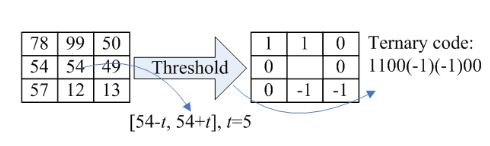
\includegraphics{ltp.JPG}
	\caption[illustration de l'opérateur basique LTP]{illustration de l'opérateur basique LTP (source : \cite{TAN})}
	\label{fig:ltp}
\end{figure}
Tan et Triggs ont par la suite divisé le code ternaire en deux codes binaires traités séparément et rassemblées ensuite lors de la phase de comparaison. Cette méthode à l'avantage de garder le système simple d'élimination
des patterns non-uniformes.
\begin{figure}[htbp]
	\centering
		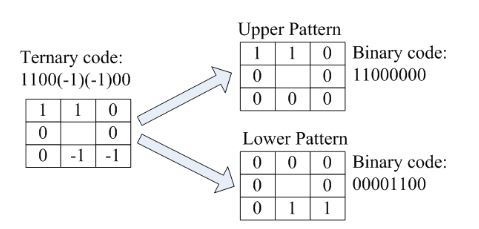
\includegraphics{tlpdivise.JPG}
	\caption{exemple de division d'un code TLP}
	\label{fig:tlp divise}
\end{figure}
\subsubsection*{Prétraitement de l'image}
La préparation de l'image s'effectue en trois étapes (cf.\cite{TAN}). 
\begin{enumerate}
	\item la correction Gamma
	\item le filtrage par différence de Gaussienne
	\item l'égalisation de contraste
\end{enumerate}
L'application de cette méthode de prétraitement à un même visage soumis à différentes conditions d'illumination
est illustrée à la figure 
\begin{figure}[htbp]
	\centering
		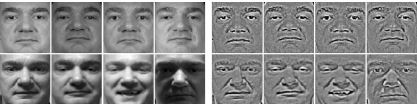
\includegraphics{pretraitement.JPG}
	\caption[Illustration du prétraitement de l'image de Tan et Triggs]{Illustration du prétraitement de l'image de Tan et Triggs (source : \cite{TAN})}
	\label{fig:pretraitement}
\end{figure}

\subsubsection*{Mesure de distance}
Tan et Triggs ont proposé une mesure de distance qui prend en compte l'organisation spatiale des LTP distribués sur l'entièreté de l'image. Les histogrammes ne sont plus utilisés. Pour comparer deux images X et Y, la méthode va regarder parmi les LTPs de même valeur de X celui qui est le plus proche et utiliser la distance qui les sépare pour incrémenter proportionnellement la distance globale. 

Autrement dit, pour un pattern de valeur k da Y, 
\begin{itemize}
	\item[\textbullet] on construit la matrice binaire $b^k_X$ qui représente la distribution des patterns k dans X.   
	\item[\textbullet] ensuite on construit les matrices $d^k_X$ de sorte qu'un élément $(i,j)$ de $d^k_X$ représente la distance entre $(i,j)$ et la position du plus proche pixel de X dont la valeur est k.
	\item[\textbullet] enfin, le calcul de la distance entre X et Y se fait par la formule
	\begin{eqnarray}
D(X,Y)=\sum_{pixels(i,j) de Y}{w(d_{X}^{k_Y(i,j)}{(i,j)})}
\label{eq20}
\end{eqnarray}
où w(d) est une fonction (à choisir) qui associe à une distance de pixel la pénalité correspondante. Tan et Triggs \cite{TAN} proposent la gaussienne $w(d)=exp^{(d/\sigma)^2/2)}$
et la troncation linéaire $w(d) = min(d; \tau)$ et disent que leurs performances sont similaires.
\end{itemize}

\section{Conclusion}
Dans ce chapitre, nous avons décrit deux méthodes de reconnaissance de visage : la méthode eigenface basée sur l'analyse en composante principale et la méthode LBP. Dans le chapitre suivant, nous mettrons ces deux algorithmes en œuvre et nous les testerons afin d'évaluer leurs performances.